\documentclass[12pt,letterpaper]{article}
\usepackage{fullpage}
\usepackage[top=1.5cm, bottom=3.5cm, left=2.2cm, right=2.2cm]{geometry}
\usepackage{amsmath,amsthm,amsfonts,amssymb,amscd, esint}
\usepackage{lastpage}
\usepackage{enumerate}
\usepackage{fancyhdr}
\usepackage{mathrsfs}
\usepackage{graphicx}
\usepackage{listings}
\usepackage{hyperref}
\usepackage[english]{babel}
\usepackage{lipsum}
\usepackage[table,xcdraw]{xcolor}
\usepackage{enumitem}
\usepackage{float}
\usepackage{chemfig}
\usepackage{yfonts}
\usepackage{tikz}
\usepackage{wrapfig}
\usepackage[normalem]{ulem}
\usepackage{multicol}
\useunder{\uline}{\ul}{}


%%%%%%%%%%%%%%% CODELISTINGS %%%%%%%%%%%%%%%%
\usepackage{listings}
\definecolor{codegreen}{rgb}{0,0.6,0}
\definecolor{codegray}{rgb}{0.5,0.5,0.5}
\definecolor{codepurple}{rgb}{0.58,0,0.82}
\definecolor{backcolour}{rgb}{0.95,0.95,0.92}

\lstdefinestyle{mystyle}{
    backgroundcolor=\color{backcolour},   
    commentstyle=\color{codegreen},
    keywordstyle=\color{magenta},
    numberstyle=\tiny\color{codegray},
    stringstyle=\color{codepurple},
    basicstyle=\ttfamily\footnotesize,
    breakatwhitespace=false,         
    breaklines=true,                 
    captionpos=t,                    
    keepspaces=true,                 
    numbers=left,                    
    numbersep=5pt,                  
    showspaces=false,                
    showstringspaces=false,
    showtabs=false,                  
    tabsize=2
}

\lstset{style=mystyle}

%%%%%%%%%%%%%%%%%%%%%%%%%%%%%%%%%%%%%%% 

\usepackage{achemso}


\newtheorem{definition}{Definition}
\newtheorem{observation}{Observation}
\newtheorem{reflection}{Reflection}
\newtheorem{PyPackage}{Package}
\newtheorem{book}{Book}

\newcommand{\HRule}[1]{\rule{\linewidth}{#1}}
\setcounter{tocdepth}{5}
\setcounter{secnumdepth}{5}

\setlength{\parindent}{0.0in}
\setlength{\parskip}{0.05in}

% Edit these as appropriate
\newcommand\course{}
\newcommand\subject{Final Degree Project}
\newcommand\degree{Bachelor's Degree in Chemistry}
\newcommand\documenttitle{Notes: AI application for azophotoswitches' optimization with pharmacological interest}
\newcommand\NetIDb{Universitat Autònoma de Barcelona}


\begin{document}
\title{\vspace{4cm} \normalsize 
		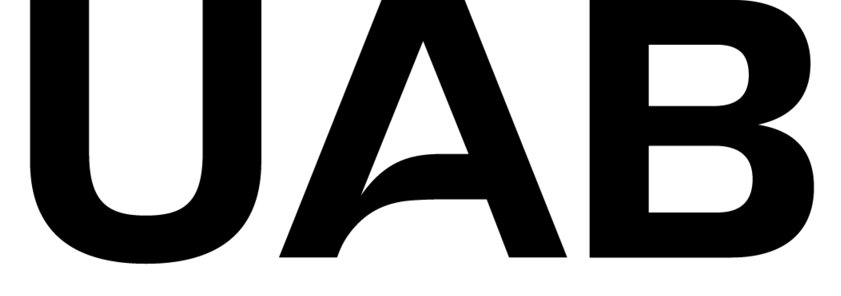
\includegraphics[width = 0.25\textwidth]{GeneralSources/UABLogo.png}\\ [0.5cm]
		\textsc{\NetIDb}\\ [2.0cm]
		\HRule{0.5pt} \\
		\LARGE \textbf{\uppercase{\documenttitle}}
		\HRule{2pt} \\ [1.5cm]
		\normalsize \begin{tabular}{rcl}  % Create a right-left column alignment
        \textsc{Author} & : & \textsc{Sergio Castañeiras Morales} \\
        \textsc{Supervisor} & : & \textsc{Miquel Moreno Ferrer} \\
        \textsc{Co-Supervisor} & : & \textsc{Àngels Gonzalez Lafont}
    \end{tabular}
    \normalsize \vspace*{5\baselineskip}
		}

\date{2024-2025}

\author{\large \textsc{\subject} \\ \textsc{\degree}}



\begin{titlepage}
\clearpage\maketitle
\thispagestyle{empty}
\end{titlepage}


\newpage
\pagestyle{fancyplain}
\headheight 35pt
\lhead{\NetIDb}    
\rhead{\subject}
\cfoot{}
\rfoot{\small\thepage}
\headsep 1.5em

%%%%%%%%%%%%%%%%%%%%%%%%%%%%%%%%%%%%%%%%%%
%%%%%%%%%%%%%%%%% DEFINITIONS %%%%%%%%%%%%%%%%%
%%%%%%%%%%%%%%%%%%%%%%%%%%%%%%%%%%%%%%%%%%

\begin{multicols}{2}
[
\section{Definitions}
]
\begin{definition}\label{definitionIC50}
$IC_{50}$: Half maximal inhibitory concentration "$IC_{50}$ is the concentration of drug required for $50\%$ inhibition. $IC_{50}$ is an operational term dependent on the assay conditions. $IC_{90}$ or $IC_{99}$ is sometimes used when complete inhibition is required. Calculation of the fractional occupancy shows that $IC_{90}$ concentration is approximately 10-fold greater than the $IC_{50}$ concentration assuming one-site binding at equilibrium with a Hill coefficient of 1."\cite{BookIC50}\\
 For this project, we aim to identify substances with the lowest possible $IC_{50}$, as our goal is to minimize the presence of foreign substances in the living organism.
\end{definition}

\begin{definition}
Molecular descriptor: "A molecular descriptor is the final result of a logical and mathematical procedure which transforms chemical information encoded within a symbolic representation of a molecule into a useful number or the result of some standardized experiment."\cite{DescriptorsBook}
\end{definition}

\begin{definition}
Constitutional Indices Descriptors: Kind of descriptor based on the constitutional composure of a molecule. They describe the basic composition of the molecule without considering its geometry or connectivity of it.
\end{definition}

\begin{definition}
Ring Descriptors: Kind of descriptor that describes the ring systems of our molecule. Quantifies properties such as the ring connectivity, type of ring (odd/even ring), aromaticy \& saturation.
\end{definition}

\begin{definition}
Topological Indices: These descriptors are based on the connectivity of atoms in a molecule without considering three-dimensional coordinates in the context of chemical graph theory. They help to describe the molecular graph (atoms as vertices, bonds as edges) using metrics like the Wiener index or the Zagreb index.
\end{definition}

\begin{definition}\label{DefinitionWienerIndices}
Wiener index: Specific topological descriptor based defined as the sum of the lengths of the shortest paths between all possible vertices in the chemical graph. Mathematically speaking, if we have a molecule with a set of $\{A_i\}_{i=0}^n$ atoms and we denote $d_B(A_i,A_j)$ the bond distance between atoms $A_i$ and $A_j$, we define the Wiener index of this molecule as,
\begin{align}
Ind_{Wiener}=\sum_{i=0}^n\sum_{j>i}^nd_B(A_i,A_j)
\end{align}
\par
For instance, if we take the n-Butane \& Isobutane  chemical graph from the Figure (\ref{figurenButaneIsobutaneGraph}) the Wiener index would be,
\begin{align}
d_B(C_1,C_2)+d_B(C_1,C_3)+d_B(C_1,C_4)\\
+ d_B(C_2,C_3)+d_B(C_2,C_4)+d_B(C_3,C_4)
\end{align}
Though this quantity is computed equally for both, n-Butane \& Isobutane, it results different due to their connectivity. For the n-Butane:
\begin{align}
1+2+3+1+2+1=10
\end{align}
While for the Isobutane:
\begin{align}
1+1+1+2+2+2=9 
\end{align}
\begin{figure}[H]
\centering
\chemfig{C_1-[1]C_2-[-1]C_3-[1]C_4}\hspace{1cm}
\chemfig{C_2-[1]C_1(-[2]C_3)-[-1]C_4}
\caption{n-Butane's \& Isobutane's  chemical graphs.}
\label{figurenButaneIsobutaneGraph}
\end{figure}
\end{definition}

\begin{definition}\label{DefinitionZagrebIndices}
Zagreb index: "For a (molecular) graph, the first Zagreb index $M_1$
 is equal to the sum of squares of the degrees of vertices, and the second Zagreb index $M_2$
 is equal to the sum of the products of the degrees of pairs of adjacent vertices." \cite{ZagrebIndicesArticle}
\end{definition}

\begin{definition}
Walk and Path Counts Descriptors: Kind of descriptor focused on counting specific paths or walks (connected sequences of atoms) in the molecular graph. For instance we can get a Walk and Path Counts Descriptor quantifying the number of Eulerian paths in a molecule's graph. They give insights into the molecule’s connectivity and complexity.
\end{definition}

\begin{definition}
Connectivity Indices: Connectivity Indices are a class of molecular descriptors that quantify the connectivity or bonding patterns between atoms in a molecule based on its topology (i.e., the molecular graph). These indices capture the degree to which atoms are connected, considering how atoms are bonded to each other rather than their physical 3D arrangement. They are typically derived from graph theory, where atoms are represented as vertices and bonds as edges.\cite{connectivityIndicesArticle}
\end{definition}

\begin{definition}
Randic Index: Specific connectivity index defined as the following,
\begin{align}
\sum_{\text{all bonds}}\frac{1}{\sqrt{d_id_j}}
\end{align}
where $d_i$ and $d_j$ denote the number of bonds of atoms $i$ and $j$ connected by a bond.\cite{RandicIndexArticle}
\end{definition}

\begin{definition}
Information Indices: Kind of descriptor based on the information theory, where the molecular structure is represented as a distribution of information (or entropy). They measure molecular complexity and diversity.
\end{definition}

\begin{definition}
2D-Matrix Based Descriptors: Kind of descriptor based in the matricidal representation of a molecule\cite{DescriptorsBookClassification}. 
\end{definition}

\begin{definition}\label{AdjacencyMatrixDefinition}
Adjacency Matrix: Specific 2D-Matrix Based Descriptor based on the matricidal representation of a molecule. If we have $\{x\}_{i=1}^n$ atoms that form our molecule, labeled from 1 to n, the adjacent matrix $A$ will contain as the element $a_{i,j}$ the number 1 if the atom $i$ and $j$ are connected and 0 otherwise. (We can also naturally add the possibilities of $a_{i,j}=2,3$ for double and triple bonds).\par
For instant in the Figure (\ref{figurenButaneIsobutaneGraph}) the adjacent matrix for the n-Butane is
\begin{align}
\text{n-Butane AM}=\begin{pmatrix}
0 & 1 & 0 & 0 \\
1 & 0 & 1 & 0 \\
0 & 1 & 0 & 1 \\
0 & 0 & 1 & 0 
\end{pmatrix}
\end{align}
Trivially we observe that the main diagonal will always be filled with 0s and the matrices will also be doubly symmetrical (respect both diagonals) due to the bounds transitivity and reflectivities properties.
\end{definition}

\begin{definition}
Distance Matrix: Specific 2D-Matrix Based Descriptor based on the computation of the shortest pathways between atoms. If we have $\{x\}_{i=1}^n$ atoms that form our molecule, labeled from 1 to n, the adjacent matrix $A$ will contain as the element $a_{i,j}$ the shortest bond distance between atom $i$ and atom $j$.\par
For instant in the Figure (\ref{figurenButaneIsobutaneGraph}) the distance matrix for the n-Butane is
\begin{align}
\text{n-Butane DM}=\begin{pmatrix}
0 & 1 & 2 & 3 \\
1 & 0 & 1 & 2 \\
2 & 1 & 0 & 1 \\
3 & 2 & 1 & 0 
\end{pmatrix}
\end{align}
\end{definition}

\begin{definition}
2D Autocorrelations: a type of molecular descriptor that quantifies the correlations between properties of atoms within a molecule based on their positions relative to one another in the molecular structure. These descriptors analyse how specific atomic properties are distributed across the molecule, capturing the spatial relationships of these properties. \par
For a given property and distance $d$, the autocorrelation is calculated by summing the products of the property values for all pairs of atoms that are separated by that distance. Mathematically, the autocorrelation  $A_d(P)$  at distance  $d$  for a property $P$  is given by,
\begin{align}
A_d(P)=\sum_{d(i,j)=d}P(i)P(j)
\end{align}
\end{definition}
\begin{definition}
Burden Eigenvalues: Kind of descriptor extracted from the Burden Matrix of a molecule\cite{BurdenIndicesArticle}, which is a modification of the adjacency matrix from the definition (\ref{AdjacencyMatrixDefinition}). 
\end{definition}

\begin{definition}
P\_VSA-like Descriptors: (Property-weighted Van der Waals Surface Area descriptors) descriptors deviated from the computation of the Van der Waals Surface of a molecule. For instance, we could talk about polarity indices, high/low electron density regions...
\end{definition}

\begin{definition}
ETA Indices: (Extended Topochemical Atom) kind of indices that capture aspects of molecular topology in conjunction with atomic properties. They are often used in the analysis of electronic properties or biological activities.\cite{DescriptorsBook}
\end{definition}

\begin{definition}
Edge Adjacency Indices: Kind of descriptor that relies on the chemical graph theory and is related to the number of bonds that each atom generates. This descriptors are tightly related to the molecule's complexity.\cite{DescriptorsBook}
\end{definition}

\begin{definition}
Fractional Group Counts (FGC): kind of molecular descriptor related to the chemical functional groups. For instance, in the case of cyclopentanone Figure (\ref{figurenCiclopentanone}), the Ketones Group Counts  is $\frac{1}{6}$, since we have 1 ketone for 6 atoms(we do not typically compute the hydrogen atoms).\cite{DescriptorsBook}
\begin{figure}[H]
\centering
\chemfig{O=*5(-----)}\hspace{1cm}
\caption{Cycloentanone's chemical graph.}
\label{figurenCiclopentanone}
\end{figure}
\end{definition}

\begin{definition}
Atom-Centered Fragments (ACF): Kind of molecular descriptor concerned about atoms separately. For a given molecule conformed by $n$ atoms, and a specific Atom-Centered Fragment descriptor, we can compute $n$ descriptors of this kind based one per each atom separately. Each descriptor describes an atom itself, its surroundings and its bounding types.\cite{DescriptorsBook}
\end{definition}

\begin{definition}
Atom-Type E-State Indices: Kind of molecular descriptor that describes the electronic state of an individual atom. Some Atom-Type E-State Indices describe the hybridisation state (e.g., $sp^2$, $sp^3$), the local bonding environment (e.g., single, double, or aromatic bonds), the presence of electronegative atoms nearby or the topological distance to other atoms in the molecule. For a given atom, a atom-type e-etate Indiex is the combination of 2 terms. The intrinsic term that depends on the atom hybridization and the perturbation term which is adjusted depending in the atom's surroundings.\cite{DescriptorsBook}
\end{definition}

\begin{definition}
Pharmacophore Descriptors: Kind of descriptor refered to the functionals groups of a given molecule and its molecular features. they describe properties such as hydrogen donation (-OH), hydrogen acceptation (C=O), Positive or negative ionizable groups (-COO$^-$)... This kind of descriptor does not worry about the molecular structure rather than the molecular properties as a hole.\cite{PharmacophoreDescriptorsBook}
\end{definition}

\begin{definition}
2D Atom Pairs: Kind of descriptor that focuses on pairs of atoms and captures information about the types of atoms involved, as well as the distance between them in a two-dimensional representation of the molecular structure.
\end{definition}

\begin{definition}
Charge descriptors: Kind of descriptor that describes a molecular charge, as a complete element as well as the composure of several elements. One of the key features of this kind of descriptors is their high dependency on dipole moment as well as the electronegativity of the atoms that it describes.
\end{definition}

\begin{definition}
Molecular Properties: The most intuitive kind of descriptor. These descriptors are the \emph{traditional features} of a substance such as it molecular weight, boiling point, solubility, density...
\end{definition}

\begin{definition}
Drug-Like Indices: These descriptors quantify how closely the molecule follows the rules for drug-likeness, such as Lipinski’s Rule of Five, which includes factors like molecular weight, hydrophobicity, and hydrogen bonding.
\end{definition}

\begin{definition}
MDE Descriptors (Molecular Distance Edge descriptors): These describe the distances between atoms in a molecule based on the molecular graph. They are useful for capturing molecular shape and spatial relationships.
\end{definition}

\begin{definition}
Chirality Descriptors: These quantify the chirality (handedness) of molecules. They reflect the 3D arrangement of atoms around chiral centers, which can influence how molecules interact with biological systems.
\end{definition}

\begin{definition}
QSAR: "Quantitative Structure–Activity Relationships are the finnal result of the
process that starts with a suitable description of molecular structures and ends with
some inference, hypothesis, and prediction on the behaviour of molecules in environmental, biological, and physico-chemical systems in analysis.\par
QSARs are based on the assumption that the structure of a molecule (for example,
its geometric, steric, and electronic properties) must contain features responsible for
its physical, chemical, and biological properties and on the ability to capture these
features into one or more numerical descriptors. By QSAR models, the biological
activity (or property, reactivity, etc.) of a new designed or untested chemical can be
inferred from the molecular structure of similar compounds whose activities
(properties, reactivities, etc.) have already been assessed."\cite{DescriptorsBookClassification}
\end{definition}

\begin{definition}
Machine Learning Model: For a given problem, Machine Learning Model is the procedure to resolve the problem in a Machine Learning like format. 
\end{definition}

\begin{definition}
The efficiency of a Machine Learning Model relies in the following quantities:
\begin{itemize}
\item True Positives (TP): number of true positives results.
\item False Positives (FP): number of false positives results.
\item True Negatives (TN): number of true negatives results.
\item Fales Negatives (FN): number of false negatives results.
\end{itemize}
\end{definition}

\begin{definition}
True Positive Rate: quantity related to a Machine Learning Model's sensitivity defined as:
\begin{align}
\frac{TP}{TP+FN}
\end{align}
\end{definition}

\begin{definition}
True Negative Rate: quantity related to a Machine Learning Model's specificity defined as:
\begin{align}
\frac{TN}{TN+FN}
\end{align}
\end{definition}

\begin{definition}
Classification Accuracy: quantity related to a Machine Learning Model's efectiveness defined as:
\begin{align}
\frac{TP+TN}{TP+FP+TN+FN}
\end{align}
\end{definition}

\begin{definition}
Matthews Correlation Coefficient: quantity related to a Machine Learning Model's prediction capacity defined as:
{\scriptsize
\begin{align}
\frac{(TP\times TN)-(FP\times FN)}{\sqrt{(TP+FP)\times(TP+FN)\times(TN+FP)\times(TN+FN)}}
\end{align}
}
A Matthews Correlation Coefficient equal to 1 stands for a perfect prediction a Matthews Correlation Coefficient equal to 0 indicates that the classifier’s predictions are no better than random guessing, and a Matthews Correlation Coefficient equal to -1 stand for a total disagreement between predictions and actual outcomes.
\end{definition}

\end{multicols}
%%%%%%%%%%%%%%%%%%%%%%%%%%%%%%%%%%%%%%%%%%
%%%%%%%%%%%%%%%% OSERVATIONS %%%%%%%%%%%%%%%%%
%%%%%%%%%%%%%%%%%%%%%%%%%%%%%%%%%%%%%%%%%%
\newpage
\begin{multicols}{2}
[
\section{Observations}
]
\begin{observation}
Machine Leaning (ML) and Artificial Intelligence (AI) are not the same concept, in fact, a ML  models are a subset of AIs. The key relies in word \emph{Learning}, generally speaking, an AI does not need to actually learn from a set of data. It can be set up within a decision tree such that logically responses with the proper answer following its criteria. \par
However a Machine Leaning Method is a kind of AI that \emph{learns} from data and evolves with the provided data.
\end{observation}
\begin{observation}
Mathematically speaking, Machine Learning methods are no different from an optimisation problem \cite{MathematicsForMachineLearningBook}.\par
Generally speaking, all ML methods seek to find a criterion to determine the quantity of a certain property of some data, which we lack knowledge of and will call the \emph{target}. In order to do so, they rely on a dataset where the sought property is already known and which establishes relationships between this property and other features of the data. Then, based on these relationships and the properties of the \emph{target}, the model searches for the position where the \emph{target} fits within the data and determines the quantity of the property, taking this placement into account within the known data.\par
For instance, we could think of standard calibration with linear regression as an ultra-simplification of a Machine Learning problem. We have a set of data (such as salt concentration in a solution) $\{x_i\}_{i=0}^n$, we also know the quantity of a certain property (such as the solution's conductivity) for each entry $x_j$, denoted as $\{f(x_i)\}_{i=0}^n$. In this example, our ML method assumes that the data and the property are linearly related and that the distance between data and the property is equivalently defined as $d(x_i, x_j) = \sqrt{x_i^2 + x_j^2}$. Hence, based on the assumption of linearity, the best possible relationship is a straight line, and the method looks for the line that minimises the distance between the line and the data.\par
Then, given a \emph{target} (for instance, a certain concentration), about which we initially lack knowledge, the method is capable of quantitatively computing the theoretical property (for instance, its conductivity) by using the fitted line representing the relationship. Consequently, this can be helpful in determining the theoretical concentration of salt needed to achieve a certain conductivity without having actual data for that concentration.\par
The \emph{learning} part (the most important part) comes from the fact that the model (the line) learns from the data. As we train our system (i.e., perform linear regression) with increasingly larger datasets, the accuracy of our model's predictions improves. Thus, we can conclude that the system is \emph{learning} from the data, which qualifies it as a Machine Learning model.\par
\end{observation}
\begin{observation}
Since we are working with molecules, our Machine Learning model will require certain parameters to determine the relationship with the property.\par
In this case, our \emph{property} (i.e., $\{f(x_i)\}_{i=0}^n$) will be the inhibition of a specific protein (COX-2), and more specifically, it will be $IC_{50}$, $IC_{90}$, or $IC_{99}$ (\ref{definitionIC50}).\par
Moreover, our \emph{parameters} (i.e., $\{x_i\}_{i=0}^n$) will be the molecular descriptors, which must be \textbf{carefully chosen}. This problem introduces additional complexities compared to the linear regression case:
\begin{itemize}
    \item We will be working with approximately $10^3$ descriptors, making this a $10^3$-dimensional problem.
    \item We want the system to automatically discard non-relevant data, as some molecules could be exceptions due to external factors.
    \item We do not assume linearity.
    \item Not all descriptors have the same distances or weights, as we will want some of them to be more relevant than others.
    \item Some descriptors will be continuous (for instance, bond distances) while others will remain discrete (for instance, topological indexes) by construction  which implies that some dimensions need to be treated differently to others.
\end{itemize}
Interestingly enough, despite these complexities, in some way, we can say that this project is not entirely different from computing a linear regression...
\end{observation}
\begin{observation}
Taking into account definitions (\ref{DefinitionWienerIndices}) and (\ref{DefinitionZagrebIndices}), we can also define a norm, denoted by $\mathcal{N}(A,B)$, which refers to the norm between molecules $A$ and $B$. For instance, this can be expressed as $\mathcal{N}(A,B) = |Ind_A - Ind_B|$, where $Ind_A$ and $Ind_B$ represent the respective indices (Wiener, Zagreb, etc.) of the molecules\footnote{Actually, any kind of norm would work, as long as it depends on the indices.}. Using this norm, we can generate a metric space that tells us how close two molecules are, based on the similarity of their indices.

In this way, we can apply the concept of “linear regression” and compute the relationship between the indices and the $IC_{50}$. This refers to one dimension, corresponding to a specific topological index. We can then extend this to consider all remaining indices (approximately $10^3$), and find the optimal position in this $10^3$-dimensional space for our resulting molecule.
\end{observation}

\begin{observation}
We have extracted all the aviable data from the \emph{ChEMBL} database with a known $IC_{50}$ value for the COX-2. After deleting  entries with the same canonical smile we remain with 4827 entries. We filter, keeping just those with a $IC_{50}\in [-1,200]$\footnote{Note that the lower constrain won't be ever surpassed by the $IC_{50}$ defintion \ref{definitionIC50}. This is equivalent to avoid constraining the data.}. Then we obtain a remaining set of 1518 entries represented in the Figure (\ref{figDataRepresentationFiltering}).
\begin{figure}[H]
\centering
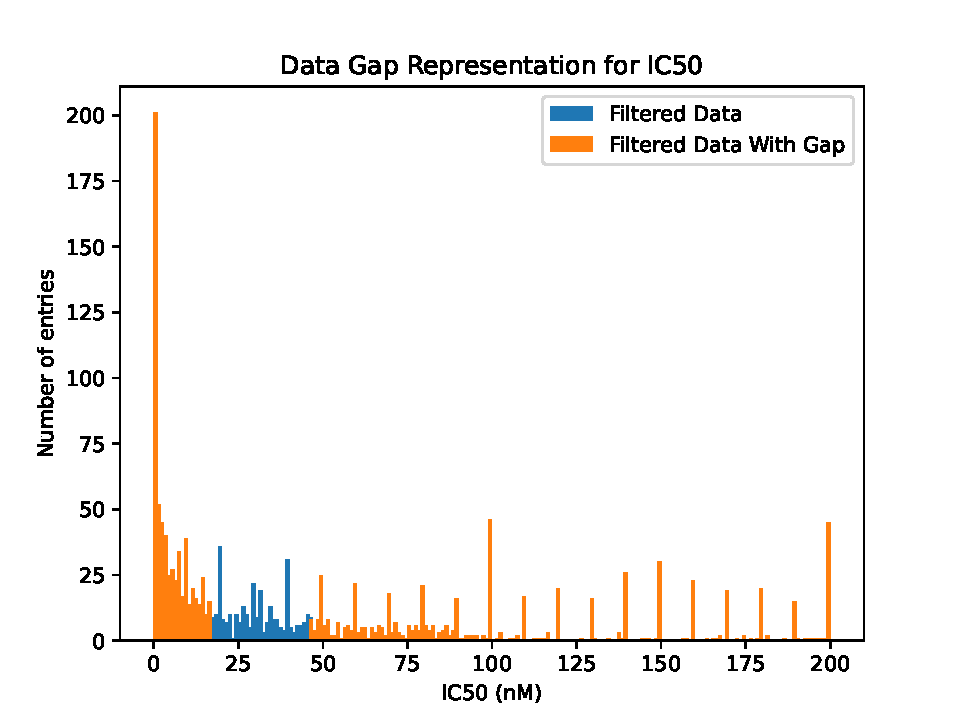
\includegraphics[width = 0.5\textwidth]{../Plots/DataGapRepresentationIC50percentageEresed20.0Gap_min_17Gap_max_47.pdf}
\caption{Data representation after the filtering.}
\label{figDataRepresentationFiltering}
\end{figure}
\end{observation}
\end{multicols}
\newpage

%%%%%%%%%%%%%%%%%%%%%%%%%%%%%%%%%%%%%%%%%%
%%%%%%%%%%%%%%%% REFLECTIONS %%%%%%%%%%%%%%%%%
%%%%%%%%%%%%%%%%%%%%%%%%%%%%%%%%%%%%%%%%%%

\begin{multicols}{2}
[
\section{Reflections}
]
\begin{reflection}
During the first meeting with Dra.González, Dr. Moreno \& Dr. Lluch a certain theme was brought up. "Wouldn't be great to actually have the wave function of the molecules?" This way we could avoid the use of descriptors and QSARs and have more accurate results. \par
Though it was a joke, it might not be a utopia someday. I believe quantum computers will be capable of this task and maybe a hundred years from today, this project could be doable working directly with the waves functions (not analytically obviously). How knows? Time will tell us.
\end{reflection}
\begin{reflection}
Fun fact, \cite{ZagrebIndicesArticle} is a mathematical article, completely apart from the chemical world but somehow we can manage to use it to describe molecules whatsoever. I believe applying knowledge from other sectors is key to evolve and reach even greater results.
\end{reflection}
\end{multicols}

%%%%%%%%%%%%%%%%%%%%%%%%%%%%%%%%%%%%%%%%%%
%%%%%%%%%%%%%%%%%% PACKAGES %%%%%%%%%%%%%%%%%
%%%%%%%%%%%%%%%%%%%%%%%%%%%%%%%%%%%%%%%%%%
\begin{multicols}{2}
[
\section{Packages}
]
\begin{PyPackage}
"Requests allows you to send HTTP/1.1 requests extremely easily. There’s no need to manually add query strings to your URLs, or to form-encode your POST data. Keep-alive and HTTP connection pooling are 100\% automatic, thanks to urllib3."
\cite{PythonPackageRequests}. We will use this package to create requests to the ChEMBL database.
\end{PyPackage}

\begin{PyPackage}
"Pandas is a Python package that provides fast, flexible, and expressive data structures designed to make working with "relational" or "labeled" data both easy and intuitive. It aims to be the fundamental high-level building block for doing practical, real world data analysis in Python. Additionally, it has the broader goal of becoming the most powerful and flexible open source data analysis / manipulation tool available in any language. It is already well on its way towards this goal"\cite{PythonPackagePandas}. We will use this package to interact with the data using a built-in Pandas class called \emph{Data Frames}.
\end{PyPackage}
\end{multicols}

%%%%%%%%%%%%%%%%%%%%%%%%%%%%%%%%%%%%%%%%%%
%%%%%%%%%%%%%%%%%% BOOKS %%%%%%%%%%%%%%%%%%%
%%%%%%%%%%%%%%%%%%%%%%%%%%%%%%%%%%%%%%%%%%

\section{Physical books in the library}
\begin{book}
Molecular descriptors for chemoinformatics. Todeschini, Roberto.; Consonni, Viviana. 2009. Volum: 2. 

Localization: Ciència i Tecnologia. 

Signatura: 54:68 Tod. 

Codi de Barres: 1501208901
\end{book}

%%%%%%%%%%%%%%%%%%%%%%%%%%%%%%%%%%%%%%%%%%
%%%%%%%%%%%%%%%%%% VARIOUS %%%%%%%%%%%%%%%%%%
%%%%%%%%%%%%%%%%%%%%%%%%%%%%%%%%%%%%%%%%%%
\newpage
\section{Various}

\begin{lstlisting}[language=C, caption=Example of a JSON file.]
{
  "page_meta": {
    "limit": 1000,
    "offset": 0,
    "total_count": 1500,
    "next": "/chembl/api/data/activity.json?limit=1000&offset=1000&target_chembl_id=CHEMBL372&standard_type=IC50",
    "previous": null
  },
  "activities": [
    {
      "activity_id": 123456789,
      "assay_chembl_id": "CHEMBL123456",
      "molecule_chembl_id": "CHEMBL25",
      "canonical_smiles": "CCOCCO",
      "standard_value": "50",
      "standard_units": "nM",
      "standard_type": "IC50",
      "target_chembl_id": "CHEMBL372",
      "assay_type": "B",
      "relation": "=",
      "document_chembl_id": "CHEMBL12345"
    },
    {
      "activity_id": 987654321,
      "assay_chembl_id": "CHEMBL654321",
      "molecule_chembl_id": "CHEMBL1095",
      "canonical_smiles": "CCCN(CC)CC",
      "standard_value": "25",
      "standard_units": "nM",
      "standard_type": "IC50",
      "target_chembl_id": "CHEMBL372",
      "assay_type": "B",
      "relation": "<",
      "document_chembl_id": "CHEMBL54321"
    }
    // More activity entries...
  ]
}
\end{lstlisting}

\newpage

%%%%%%%%%%%%%%%%%%%%%%%%%%%%%%%%%%%%%%%%%%
%%%%%%%%%%%%%%%% BIBLIOGRAPHY %%%%%%%%%%%%%%%%%
%%%%%%%%%%%%%%%%%%%%%%%%%%%%%%%%%%%%%%%%%%

% \bibliographystyle{achemso}
\bibliography{references} 
%%%%%%%%


\end{document}